%!TEX TS-program = xelatex
\documentclass[12pt, a4paper, oneside]{article}

% пакеты для математики
\usepackage{amsmath,amsfonts,amssymb,amsthm,mathtools}  
\mathtoolsset{showonlyrefs=true}  % Показывать номера только у тех формул, на которые есть \eqref{} в тексте.

\usepackage[english, russian]{babel} % выбор языка для документа
% \usepackage[utf8]{inputenc}          % utf8 кодировка

% Основные шрифты 
\usepackage{fontspec}         
\setmainfont{Linux Libertine O}  % задаёт основной шрифт документа

% Математические шрифты 
\usepackage{unicode-math}     
\setmathfont[math-style=upright]{[Neo Euler.otf]} 


%%%%%%%%%% Работа с картинками и таблицами %%%%%%%%%%
\usepackage{graphicx} % Для вставки рисунков                
\usepackage{graphics}
\graphicspath{{images/}{pictures/}}   % папки с картинками

\usepackage{wrapfig}    % обтекание рисунков и таблиц текстом

\usepackage{booktabs}   % таблицы как в годных книгах
\usepackage{tabularx}   % новые типы колонок
\usepackage{tabulary}   % и ещё новые типы колонок
\usepackage{float}      % возможность позиционировать объекты в нужном месте
\renewcommand{\arraystretch}{1.2}  % больше расстояние между строками


%%%%%%%%%% Графики и рисование %%%%%%%%%%
\usepackage{tikz, pgfplots}  % языки для графики
\pgfplotsset{compat=1.16}

\usepackage{todonotes} % для вставки в документ заметок о том, что осталось сделать
% \todo{Здесь надо коэффициенты исправить}
% \missingfigure{Здесь будет Последний день Помпеи}
% \listoftodos --- печатает все поставленные \todo'шки


%%%%%%%%%% Внешний вид страницы %%%%%%%%%%

\usepackage[paper=a4paper, top=20mm, bottom=15mm,left=20mm,right=15mm]{geometry}
\usepackage{indentfirst}    % установка отступа в первом абзаце главы

\usepackage{setspace}
\setstretch{1.15}  % межстрочный интервал
\setlength{\parskip}{4mm}   % Расстояние между абзацами
% Разные длины в LaTeX: https://en.wikibooks.org/wiki/LaTeX/Lengths

% свешиваем пунктуацию
% теперь знаки пунктуации могут вылезать за правую границу текста, при этом текст выглядит ровнее
\usepackage{microtype}

% \flushbottom                            % Эта команда заставляет LaTeX чуть растягивать строки, чтобы получить идеально прямоугольную страницу
\righthyphenmin=2                       % Разрешение переноса двух и более символов
\widowpenalty=300                     % Небольшое наказание за вдовствующую строку (одна строка абзаца на этой странице, остальное --- на следующей)
\clubpenalty=3000                     % Приличное наказание за сиротствующую строку (омерзительно висящая одинокая строка в начале страницы)
\tolerance=10000     % Ещё какое-то наказание.

% мои цвета https://www.artlebedev.ru/colors/
\definecolor{titleblue}{rgb}{0.2,0.4,0.6} 
\definecolor{blue}{rgb}{0.2,0.4,0.6} 
\definecolor{red}{rgb}{1,0,0.2} 
\definecolor{green}{rgb}{0,0.6,0} 
\definecolor{purp}{rgb}{0.4,0,0.8} 

% цвета из geogebra 
\definecolor{litebrown}{rgb}{0.6,0.2,0}
\definecolor{darkbrown}{rgb}{0.75,0.75,0.75}

% Гиперссылки
\usepackage{xcolor}   % разные цвета

\usepackage{hyperref}
\hypersetup{
	unicode=true,           % позволяет использовать юникодные символы
	colorlinks=true,       	% true - цветные ссылки
	urlcolor=blue,          % цвет ссылки на url
	linkcolor=red,          % внутренние ссылки
	citecolor=green,        % на библиографию
	breaklinks              % если ссылка не умещается в одну строку, разбивать её на две части?
}

% меняю оформление секций 
\usepackage{titlesec}
\usepackage{sectsty}

% меняю цвет на синий
\sectionfont{\color{titleblue}}
\subsectionfont{\color{titleblue}}

% выбрасываю нумерацию страниц и колонтитулы 
\pagestyle{empty}

% синие круглые бульпоинты в списках itemize 
\usepackage{enumitem}

\definecolor{itemizeblue}{rgb}{0, 0.45, 0.70}

\newcommand*{\MyPoint}{\tikz \draw [baseline, fill=itemizeblue, draw=blue] circle (2.5pt);}

\renewcommand{\labelitemi}{\MyPoint}

% расстояние в списках
\setlist[itemize]{parsep=0.4em,itemsep=0em,topsep=0ex}
\setlist[enumerate]{parsep=0.4em,itemsep=0em,topsep=0ex}


%%%%%%%%%% Свои команды %%%%%%%%%%

% Математические операторы первой необходимости:
\DeclareMathOperator{\sgn}{sign}
\DeclareMathOperator*{\argmin}{arg\,min}
\DeclareMathOperator*{\argmax}{arg\,max}
\DeclareMathOperator{\Cov}{Cov}
\DeclareMathOperator{\Var}{Var}
\DeclareMathOperator{\Corr}{Corr}
\DeclareMathOperator{\E}{\mathop{E}}
\DeclareMathOperator{\Med}{Med}
\DeclareMathOperator{\Mod}{Mod}
\DeclareMathOperator*{\plim}{plim}

% команды пореже
\newcommand{\const}{\mathrm{const}}  % const прямым начертанием
\newcommand{\iid}{\sim i.\,i.\,d.}  % ну вы поняли...
\newcommand{\fr}[2]{\ensuremath{^{#1}/_{#2}}}   % особая дробь
\newcommand{\ind}[1]{\mathbbm{1}_{\{#1\}}} % Индикатор события
\newcommand{\dx}[1]{\,\mathrm{d}#1} % для интеграла: маленький отступ и прямая d

% одеваем шапки на частые штуки
\def \hb{\hat{\beta}}
\def \hs{\hat{s}}
\def \hy{\hat{y}}
\def \hY{\hat{Y}}
\def \he{\hat{\varepsilon}}
\def \hVar{\widehat{\Var}}
\def \hCorr{\widehat{\Corr}}
\def \hCov{\widehat{\Cov}}

% Греческие буквы
\def \a{\alpha}
\def \b{\beta}
\def \t{\tau}
\def \dt{\delta}
\def \e{\varepsilon}
\def \ga{\gamma}
\def \kp{\varkappa}
\def \la{\lambda}
\def \sg{\sigma}
\def \tt{\theta}
\def \Dt{\Delta}
\def \La{\Lambda}
\def \Sg{\Sigma}
\def \Tt{\Theta}
\def \Om{\Omega}
\def \om{\omega}

% Готика
\def \mA{\mathcal{A}}
\def \mB{\mathcal{B}}
\def \mC{\mathcal{C}}
\def \mE{\mathcal{E}}
\def \mF{\mathcal{F}}
\def \mH{\mathcal{H}}
\def \mL{\mathcal{L}}
\def \mN{\mathcal{N}}
\def \mU{\mathcal{U}}
\def \mV{\mathcal{V}}
\def \mW{\mathcal{W}}

% Жирные буквы
\def \mbb{\mathbb}
\def \RR{\mbb R}
\def \NN{\mbb N}
\def \ZZ{\mbb Z}
\def \PP{\mbb{P}}
\def \QQ{\mbb Q}


%%%%%%%%%% Теоремы %%%%%%%%%%
\theoremstyle{plain} % Это стиль по умолчанию.  Есть другие стили.
\newtheorem{theorem}{Теорема}[section]
\newtheorem{result}{Следствие}[theorem]
% счётчик подчиняется теоремному, нумерация идёт по главам согласованно между собой

% убирает курсив и что-то еще наверное делает ;)
\theoremstyle{definition}         
\newtheorem*{definition}{Определение}  % нумерация не идёт вообще


%%%%%%%%%% Задачки и решения %%%%%%%%%%
\usepackage{etoolbox}    % логические операторы для своих макросов
\usepackage{environ}
\newtoggle{lecture}

\newcounter{problem}%[section]  % счётчик для упражнений 

\renewcommand{\theproblem}{\arabic{problem}}

\newenvironment{problem}[1]{
\addtocounter{problem}{1}\noindent{ \color{titleblue} \large \bfseries Упражнение~\theproblem~#1 \vspace{1ex} \newline}
}{ }

% Окружение, чтобы можно было убирать решения из pdf
\NewEnviron{solution}{%
  \iftoggle{lecture}
    {\noindent \textbf{\large Решение:} \vspace{1ex} \newline \BODY}
    {}%
  }
  
% выделение по тексту важных вещей
\newcommand{\indef}[1]{\textbf{ \color{green} #1}} 

\begin{document} % Конец преамбулы, начало файла

% Если переключить в false, все solution исчезнут из pdf
\toggletrue{lecture}
%\togglefalse{lecture}

\section*{Семинар 5: Регрессия}

В этом семинаре мы впервые столкнёмся с настоящим машинным обучением и попробуем понять что стоит за его магией. В ручной части семинара мы пойдём по следующему  плану: 

\begin{enumerate}
\item разберёмся чем классификация отличается от регрессии, сформулируем задачу регрессии и поймём её специфику;
\item поймём с помощью каких метрик можно оценить качество прогноза в случае регрессии и попробуем разобраться какой смысл стоит за этими метриками;
\item разберёмся как выглядит простейшая линейная модель регрессии;
\item на пальцах прикинем как она обучается.
\end{enumerate}

\begin{problem}{(ставим задачу)}
Представьте себе, что у вас есть паблик с мемами. \indef{Вы --- Хозяин мемов.} Как и любой другой Хозяин мемов, вы любите лайки под мемами. Возникает желание привлечь в паблик целевую аудиторию, которая будет ставить под мемы лайки. Для этого вы хотите запустить рекламную кампанию паблика. Ясное дело, что рекламу хочется показывать не всем подряд,  а только подходящим людям. 

У вас есть данные по профилям всех тех людей, которые уже ставили в паблике лайки. По этим данным вам хочется построить модель, которая могла бы предсказать подходит ли конкретный человек для вашей рекламной компании (поставил бы ли он в паблик лайк, если бы был на него подписан). 

\begin{enumerate}
\item[а)] Сформулируйте задачу машинного обучения. Какой должна быть целевая переменная, чтобы перед вами была задача классификации. Какой должна быть целевая переменная, чтобы это была задача регрессии? 

\item[б)] Какие факторы из профилей вы бы использовали, чтобы спрогнозировать подходит ли человек для рекламной кампании?

\item[в)] Приведите ещё парочку примеров задачи классификации и задачи регрессии. 
\end{enumerate}
\end{problem}

\begin{solution}
Если мы будем пытаться спрогнозировать факт лайка (пользователь поставил хотя бы один лайк в паблик), то мы будем решать задачу классификации, так как мы стараемся предсказать бинарную переменную (либо поставил, $1$, либо нет, $0$). Если мы будем пытаться спрогнозировать непрерывную переменную: количество лайков, которое пользователь поставил в паблике, то мы будем решать задачу регрессии. 

В качестве факторов для прогноза можно использовать абсолютно любую информацию из профилей: пол, возраст, есть ли аватар, как часто человек что-то репостит, на какие другие похожие паблики он подписан и т.п.  Правда не факт, что все эти переменные окажутся полезными. 

\indef{Классификация:} предсказание оттока клиентов, вернёт ли человек кредит, болен ли человек, содержит ли письмо спам, мошенническая ли транзакция,  сделает ли человек клик,  поставит ли лайк и т.д.

\indef{Регрессия:} предсказание цен, спроса, выручки, валютного курса,  ВВП страны, инфляции, качества вина, уровня преступности (число преступлений на душу населения) и т.д.
\end{solution}


\begin{problem}{(качество прогноза)}
Добрыня, Алёша и Илья смотрят мемы и ставят на них лайки. Мы пытаемся предсказать сколько лайков они оставят под мемами на основе поведения их однокурсников. Для этого мы оценили регрессию. Ну и она нам напредсказывала, что парни поставят $4$, $20$ и $110$ лайков. В реальности они поставили $5$, $10$ и $100$ лайков. Возникает вопрос: насколько сильно наша модель ошиблась в прогнозировании. 

Что такое $MAE$, $MSE$, $RMSE$ и $MAPE$?  Посчитайте для модели все четыре метрики качества.
\end{problem}

\begin{solution}
Попробуем посчитать основные метрики, которые встречаются для регрессии. 
\begin{itemize}
	\item \indef{MAE (mean absolute error), средняя абсолютная ошибка}
	
	Первой очевидной метрикой качества будет просто взять и просуммировать все ошибки модели. Так, в случае Добрыни ошибка оказалась $|5 - 4| = |1| = 1$. Модуль от ошибки берётся, потому что можно ошибаться в разные стороны. Например, если бы не было модуля, для Алёши ошибка составила бы $10 - 20 = -10$. Потом нам надо было бы сложить две ошибки и мы получили бы $9$. Ошибка в $9$ лайков. А это неправда, потому что мы ошиблись в $11$ лайков. Поэтому берётся модуль. 
	
	Средняя абсолютная ошибка для парней составит: 
	
	$$ 
	\frac{1}{3} \cdot (|5 - 4| + |10 - 20| + |100 - 110|) = 7
	$$
	
	В среднем мы ошибаемся на $7$ лайков. Формула для поиска средней абсолютной ошибки в общем виде выглядит вот так: 
	
	$$
	MAE = \frac{1}{n}\sum_{i=1}^{n} |y_i - \hat{y}_i|.
	$$
	 
	 Можно нарисовать $MAE$ на картинке. По оси $x$ отложим ошибку прогноза. В случае Добрыни это $5-4 = 1$. По оси $y$ будем откладывать то, насколько сильный штраф мы накладываем за такую ошибку. В случае $MAE$ штраф за ошибку в $1$ равен $1$. То есть мы получаем прямую под углом в $45$ градусов. В отрицательную сторону ошибка также штрафуется один к одному. График выглядит, как галочка. 

\begin{center}
\begin{tikzpicture}[line cap=round,line join=round,x=1.0cm,y=1.0cm]

	%\draw [xstep=1.0cm,ystep=1.0cm] (-4,-1) grid (4,4);
    \draw [->,line width=1.5pt] (-3.5,0) -- (3.5,0);
    \draw [->,line width=1.5pt] (0,-0.5) -- (0,4);

	\draw [line width=2.pt,color=blue] (0,0)-- (3,3);
    \draw [line width=2.pt,color=blue] (0,0)-- (-3,3);
    
    \draw[thick,dashed,color=blue] (1,0)-- (1,1);
    \draw[thick,dashed,color=blue] (0,1)-- (1,1);
    \draw (0,1) node[anchor=east] {$1$};
    \draw (1,0) node[anchor=north] {$1$};
    
    \draw[thick,dashed,color=blue] (-2,0)-- (-2,2);
    \draw[thick,dashed,color=blue] (0,2)-- (-2,2);
    \draw (0,2.3) node[anchor=east] {$2$};
    \draw (-2,0) node[anchor=north] {$-2$};

    \draw (2,-0.2) node[anchor=north west] {ошибка прогноза};
    \draw (-1,4.8) node[anchor=north west] {потери (MAE)};
\end{tikzpicture}
\end{center}
	 	
\item \indef{квантильная ошибка}

Один из минусов MAE в том, что мы одинаково нелюбим перепрогноз и недопрогноз. В реальности цена этих двух ошибок может быть разной. Мы можем это учесть. Представим себе ситуацию, что Хозяин мемов очень сильно обижается, если мы прогнозируем ему больше лайков, чем получается в реальности. Если мы прогнозируем меньше, чем в реальности, он также обижается, но чуть-чуть. В общем, когда мы делаем перепрогноз, он обижается в $2$ раза сильнее. Тогда ошибку можно посчитать по формуле: 

$$ 
\frac{1}{3} \cdot (|5 - 4| + 2 \cdot |10 - 20| + 2 \cdot |100 - 110|) = 13.6 
$$

То есть мы умножили перепрогнозы на два. На самом деле в реальности коэффициенты могут быть и другими. Чаще всего они берутся из всяких денежных соображений. В случае, если бы мы прогнозировали не лайки, а продажи в магазине, недопрогноз спроса мог бы для нас быть серьёзнее из-за потери кучи денег в виде лояльных клиентов. Насколько он страшнее мы могли бы попытаться померить в деньгах. Такая неравномерная ошибка обычно называется \indef{квантильной ошибкой.}

Если мы решим нарисовать такую ошибку на картинке, наша галочка чуть-чуть покорёжится. 
	
\begin{center}
\begin{tikzpicture}[line cap=round,line join=round,x=1.0cm,y=1.0cm]

	%\draw [xstep=1.0cm,ystep=1.0cm] (-4,-1) grid (4,4);
    \draw [->,line width=1.5pt] (-3.5,0) -- (3.5,0);
    \draw [->,line width=1.5pt] (0,-0.5) -- (0,4);

	\draw [line width=2.pt,color=blue] (0,0)-- (2,4);
    \draw [line width=2.pt,color=blue] (0,0)-- (-3,3);
    
    \draw[thick,dashed,color=blue] (1,0)-- (1,2);
    \draw[thick,dashed,color=blue] (0,2)-- (1,2);
    \draw (0,2) node[anchor=east] {$2$};
    \draw (1,0) node[anchor=north] {$1$};
    
    \draw[thick,dashed,color=blue] (-1,0)-- (-1,1);
    \draw[thick,dashed,color=blue] (0,1)-- (-1,1);
    \draw (0,1.3) node[anchor=east] {$1$};
    \draw (-1,0) node[anchor=north] {$-1$};

    \draw (2,-0.2) node[anchor=north west] {ошибка прогноза};
    \draw (-2.5,4.8) node[anchor=north west] {потери (квантильная ошибка)};
\end{tikzpicture}
\end{center}

Увидели? Теперь, если мы ошибаемся на единицу направо, то есть происходит перепрогноз, мы несём потери размером $2$. Если мы ошибаемся на единицу налево, то есть происходит недорогноз, мы несём потери в $1$. Получается, что любой сдвиг вправо в плане ошибки для нас в два раза хуже, чем влево. Чем больше коэффициент перед ошибкой, тем резче дисбаланс в ошибках для нас. В общем виде квантильную ошибку можно записать вот так: 

$$
QE = \frac{1}{n}\sum_{i=1}^n \rho(y_i - \hat y_i),
$$

где функция $\rho(y_i - \hat y_i)$ это 

$$
\rho(y_i - \hat y_i) = \begin{cases} \alpha_1 \cdot (y_i - \hat y_i), \text{ если } y_i \ge \hat y_i \\  \alpha_2 \cdot (\hat y_i - y_i), \text{ если } y_i < \hat y_i  \end{cases}. 
$$

Буквы $\a_1$ и $\a_2$ означают какие-то штрафы. В нашем случае это $1$ и $2$. 

\item \indef{Кусочно-линейная функция потерь} 
	
Можно немного модернизировать квантильную ошибку и превратить её в кусочно-линейную функцию потерь. Такая функция неплохо подойдёт для задачи прогнозирования продаж. 


\begin{center}
\begin{tikzpicture}[line cap=round,line join=round,x=1.0cm,y=1.0cm]

	%\draw [xstep=1.0cm,ystep=1.0cm] (-4,-1) grid (4,4);
    \draw [->,line width=1pt] (-4,0) -- (4,0);
    \draw [->,line width=1pt] (0,-0.5) -- (0,4);
    
    \draw [fill=blue] (0,0) circle (2pt);
 	\draw [line width=2.pt,color=blue] (0,0)-- (2,1);
    \draw [line width=2.pt,color=blue] (2,1)-- (3,4);
    \draw [fill=blue] (2.,1.) circle (2pt);
    \draw[thick,dashed,color=blue] (2,-0.5)-- (2,4);
    \draw (2,-0.5) node[anchor=north] {$50$};
    
    \draw [line width=2.pt,color=blue] (0,0)-- (-1.5,0);
    \draw [line width=2.pt,color=blue] (-1.5,0)-- (-4,1);
    \draw [fill=blue] (-1.5,0) circle (2pt);
    \draw[thick,dashed,color=blue] (-1.5,-0.5)-- (-1.5,4);
    \draw (-1.8,-0.5) node[anchor=north] {$-100$};

    \draw (2.1,1.5) node[anchor=north west] {\small просрочка};
    \draw (0,1.5) node[anchor=north west] {\small хранение};
    \draw (-1.5,1.5) node[anchor=north west] {\small запасы};
    \draw (-3.8,1.5) node[anchor=north west] {\small лояльность};

    \draw (2.5,-0.2) node[anchor=north west] {ошибка прогноза};
    \draw (-0.7,4.8) node[anchor=north west] {потери};
\end{tikzpicture}
\end{center}

Если мы спрогнозировали слишком маленький спрос, мы произведём мало товара и его не хватит всем покупателям. Идём по оси $x$ налево. Поначалу наш косяк смогут закрыть резервы со склада. И мы не будем терпеть никаких убытков. Но рано или поздно они подойдут к концу. Предположим, что на складе хранится $100$ единиц товара. Тогда, если мы пробьём своей ошибкой его объём, получится не очень хорошая ситуация. 

Приходят к нам потребители и говорят: мы хотим телевизор. А у нас нет. На складе пусто. Ну потребитель и говорит нам, что пошел в другой магазин, раз у нас пусто. Мы теряем лояльность потребителя и, скорее всего, в следующий раз он пойдёт сразу в другой магазин. Это страшно. Поэтому, начиная с ошибки в $-100$, у нас появляются потери. Насколько крутыми они будет, зависит от того, как быстро тает лояльность пользователя. Это нужно как-то оценивать по данным. И это отдельная задача. 

Если мы спрогнозировали слишком большой спрос, мы наклепаем лишнего товара. Движемся по оси $x$ направо. Если мы произвели не особо много лишнего, можно положить весь товар на склад до лучших времён. Мы будем нести издержки на хранение. У кривой потерь будет один угол. Если товара было произведено слишком много, часть просочится. Мы должны будем выкидывать товар на помойку и угол у потерь будет более крутым. Например, на картинке, мы нарисовали потери так, что если перепрогноз был больше, чем на $50$ единиц, то будет просрочка. Откуда взять это число? Опять же надо посмотреть на реальные данные и понять начиная с какой отметки товар точно будет портиться. 

Для кусочно-линейной функции потерь можно придумать довольно большое количество разных ситуаций и углов в зависимости от бизнесовой составляющей вашей задачки. 

\item \indef{MSE (mean squared error), средняя квадратичная ошибка.} 

Все три метрики, о которых мы уже поговорили, линейно накидывают потери за ошибку. А, что если мы хотим штрафовать большие потери сильнее, при этом ещё и нелинейно? Тут нам на помощь приходит штука по названием \indef{средняя квадратичная ошибка.} Считается по формуле 

$$ MSE = \frac{1}{n}\sum_{i=1}^{n} (y_i - \hat{y}_i)^2.$$

Для нашей ситуации она составит 

$$
MSE = \frac{1}{3} \cdot(  (5-4)^2 + (10 - 20)^2 + (100 - 110)^2) = 67
$$ 

Посчитали, на формулу посмотрели. Теперь давайте разбираться какой в этом смысл. Смысл в том, чтобы штрафовать за большие ошибки сильнее, чем за маленькие. Если мы ошиблись на 5 лайков, то в потери войдёт 25. Если мы ошиблись на 10 лайков, то в потери войдёт 100. Чем выше ошибка, тем сильнее потери. 

Вы можете сказать мне:  <<А зачем? Квантильная ошибка делает то же самое!>> Не совсем. В примере, на который мы смотрели выше, мы каждый раз умножали квантильную ошибку на одно и то же число, $2$. То есть за ошибку в $5$ лайков мы бы понесли потери размером $10$.  За ошибку в $10$ лайков мы бы понесли потери размером $20$. То есть в два раза больше. В случае MSE потери получились $25$ и $100$. То есть в $4$ раза больше. 

В квантильной ошибке пропорция между потерями всегда одинаковая, а в квадратичной ошибке она постоянно увеличивается.  Давайте нарисуем на картинке. 

\begin{center}
\begin{tikzpicture}[line cap=round,line join=round,x=1.0cm,y=1.0cm]

	%\draw [xstep=1.0cm,ystep=1.0cm] (-4,-1) grid (4,4);
    \draw [->,line width=1.5pt] (-3.5,0) -- (3.5,0);
    \draw [->,line width=1.5pt] (0,-0.5) -- (0,4.5);
    
    \draw [blue, thick, domain=-2.2:2.2] plot (\x, {\x*\x});
    
    \draw[thick,dashed,color=blue] (1,0)-- (1,1);
    \draw[thick,dashed,color=blue] (0,1)-- (1,1);
    \draw (0,1) node[anchor=east] {$1$};
    \draw (1,0) node[anchor=north] {$1$};
    
    \draw[thick,dashed,color=blue] (2,0)-- (2,4);
    \draw[thick,dashed,color=blue] (0,4)-- (2,4);
    \draw (0,4) node[anchor=east] {$4$};
    \draw (2,0) node[anchor=north] {$2$};

    \draw (2,-0.2) node[anchor=north west] {ошибка прогноза};
    \draw (-1,5.3) node[anchor=north west] {потери (MSE)};
\end{tikzpicture}
\end{center}
	
Ошиблись на один лайк? Потери $1$. На два лайка? Потери $4$. На три лайка? Потери $9$. Потери каждый раз всё больше. Такова природа этой ошибки. Если вы ещё не забыли в дисперсии была такая же логика. 

У $MSE$ есть проблемы с выбросами. Она очень резко реагирует на них и штрафует за их наличие очень сильно.  Если вы знаете, что у вас в данных выбросы и хотите использовать $MSE$, от них нужно избавиться. 

\textbf{Вопрос:} а чувствительна ли к выбросам  $MAE$? \textbf{Ответ:} нет, потому что там идёт сумма по модулю и нет более жёсткого штрафа за более высокие отклонения.

\item \indef{RMSE (root mean squared error)} 

Когда мы говорили про $MAE$, мы выяснили, что потери в её случае измеряются в лайках (ну или в телевизорах). Для $MSE$ мы каждое слагаемое возводим в квадрат, и итоговая сумма измеряется в квадратных лайках. Или в квадратных телевизорах. Ну или на худой конец в квадратных попугаях. Можно извлечь из $MSE$ квадратный корень, чтобы избавиться от квадрата \indef{(снова как в случае дисперсии и среднего квадратичного отклонения).} Тогда получится новая ошибка, $RMSE$. Посчитаем её для нашей ситуации: 

$$
RMSE = \sqrt{MSE} = \sqrt{67}  \approx 8.19
$$

Из-за того, что более большие ошибки для нас страшнее, $RMSE$ обычно получается больше, чем $MAE$. 

\item \indef{MAPE (mean absolute percentage error)} 

Последний герой нашей задачки про метрики. Часто для нас принципиальным является не то, на сколько лайков мы ошиблись, а то на сколько процентов мы ошиблись. Метрика, которая отлавливает процентную ошибку, называется $MAPE$ (mean absolute percentage error), средняя абсолютная процентная ошибка. 

$$
MAPE = \frac{1}{n} \sum_{i=1}^n \frac{|y_i - \hat{y}_i|}{y_i}
$$

Если вы предсказали  $1$, а в реальности было  $10$ --- это не то же самое, что вы предсказали  $1000$, а в реальности было $1009$. С точки зрения МАЕ или MSE, это две совершенно одинаковые ошибки. А если вас интересует, в среднем на сколько процентов вы ошибаетесь, то это отражает МАРЕ.  В первой ситуации мы ошиблись на $100 \cdot \frac{|1 - 10|}{10} = 90$ процентов от реального результата. Во второй ситуации на $100 \cdot \frac{|1000 - 1010|}{1009} \approx 1$ процент от реального результата.  Часто MAPE используют в финансах. Там обычно для нас важен процент, который мы получаем в качестве дохода. Давайте посчитаем метрику для нашей выборки.

$$
MAPE = 100\cdot \frac{1}{3} \cdot\left( \frac{|5 - 4|}{5} + \frac{|10 -20|}{10} + \frac{|100 - 110|}{100} \right) =  43 \% 
$$

В среднем при каждом прогнозе мы ошибаемся на $43\%$ от реального результата. 

Этого набора метрик нам для начала хватит. На практике часто используются разные другие метрики. Про них можно поподробнее почитать, например \href{https://alexanderdyakonov.files.wordpress.com/2018/10/book_08_metrics_12_blog1.pdf}{в книге Дьяконова (тут гиперссылка, тыкнете её и перейдёте в книгу).} Правда там для вас будет посложнее в плане математики.
\end{itemize} 
\end{solution}


\begin{problem}{(как выглядит модель)}
Предположим, Олег хочет купить автомобиль и считает сколько денег ему нужно для этого накопить\footnote{Сделано по мотивам статьи "Машинное обучение для людей", прочтите её: \url{https://vas3k.ru/blog/machine_learning/}}. Он пересмотрел десяток объявлений в интернете и увидел, что новые автомобили стоят около $20 000$, годовалые — примерно $19 000$, двухлетние — $18 000$ и так далее.

В уме Олег-аналитик выводит формулу: адекватная цена автомобиля начинается от $20 000$ и падает на $1000$ каждый год, пока не упрётся в $10 000$. Олег сделал то, что в машинном обучении называют регрессией --- предсказал цену по известным данным. Давайте попробуем повторить подвиг Олега.

\begin{enumerate}
	\item[а)] Как выглядит формула в случае Олега?
	\item[б)] За сколько продать старый айфон? Придумайте формулу для предсказания. Проинтерпретируйте каждый коэффициент в ней. 
	\item[в)] Сколько одежды брать с собой в путешествие?  Придумайте формулу для предсказания. Проинтерпретируйте каждый коэффициент в ней. 
	\item[г)] Сколько шашлыка брать на дачу? Как выглядит формула?
	\item[д)] Сколько брать шашлыка, если есть толстый друг? Как можно назвать толстого друга в терминах машинного обучения? Испортит ли толстый друг формулу?
\end{enumerate}

Было бы удобно иметь формулу под каждую проблему на свете. Но взять те же цены на автомобили: кроме пробега есть десятки комплектаций, разное техническое состояние, сезонность спроса и еще столько неочевидных факторов, которые Олег, даже при всём желании, не учел бы в голове. Люди тупы и ленивы — надо заставить вкалывать роботов.
\end{problem}

\begin{solution}
	\begin{enumerate}
		\item[а)]  Формула Олега: $y_i = 20000 - 1000 \cdot x_i$, где $y_i$--- цена машины, $x_i$ --- её возраст. Если бы мы собрали данные о машинах и загнали их в компьютер, нам нужно было бы оценить модель
		
		\[ y_i = \beta_0 + \beta_1 \cdot  x_i.\]
		
		Коэффициент $\beta_0$ отражает базовую стоимость машины, а $\beta_1$ то, насколько она дешевеет с каждым годом. 
		
		\item[б)]  Я не знаю, к чему мы пришли при обсуждении на семинаре, но скорее всего к чему-то похожему на случай Олега. 
		
		\item[в)]  Это зависит как минимум от двух вещей: длительности поездки и пола. Девушкам обычно нужно больше вещей. Формула для обучения может выглядеть, например, вот так: 
		
		\[ 
		y_i = \beta_0 + \beta_1 \cdot  x_i + \beta_2 \cdot femail_i,
		\]
		
		где $x_i$ --- срок поездки, а $femail_i$ принимает значение $1$, если путешественник --- девушка. Тогда коэффициент $\beta_1$ будет говорить сколько дополнительной одежды нам надо взять, если срок путешествия увеличивается на один день. Коэффициент $\beta_0$ --- какое-то базовое количество одежды, которое надо взять с собой в любом случае (ну, например она надета на нас). Коэффициент $\beta_2$ будет говорить сколько одежды надо взять с собой в любом случае дополнительно, если вы девушка. То есть для парней надо взять с собой полюбак $\beta_0$ одежды, а для девушек $\beta_0 + \beta_2$ одежды.
		
		Можно ещё сильнее усложнить формулу и получить 
		
		\[ 
		y_i = \beta_0 + \beta_1 \cdot  x_i + \beta_2 \cdot femail_i + \beta_3 \cdot femail_i \cdot x_i,
		\]		
		
		Коэффициент $\beta_3$ в таком уравнении будет говорить на сколько единиц одежды надо взять больше, на каждый дополнительный день, если путешественник --- девушка. 
		
		\item[в)]   Это зависит от числа людей и числа дней, на которое мы едем на дачу. Наверное логично было бы брать полкило на человека в день, то есть $y_i = 0.5 \cdot x_i \cdot z_i$, где $x_i$ --- число человек, $z_i$ --- число дней. 
		
		Да, да. Это тоже модель! И она нелинейная. Никто не обещал, что будет легко. Можно при желании превратить её в линейную (линеаризовать). Обычно это делается с помощью логарифмирования: 
		
		\[ \ln y_i = \ln 0.5 + \ln x_i + \ln z_i.\]
		
		В данном случае мы подобрали все коэффициенты из головы, задействовав свой природный оцениватель. Другой путь: собрать данные о поездках на дачу и заставить компьютер оценить модель: 
		
		\[ \ln y_i = \beta_0 + \beta_1 \cdot \ln x_i + \beta_2 \cdot \ln z_i.\]
		
		Такие модели, записанные в логарифмах интерпретируются чуть сложнее линейных. Они интерпретируются в процентах. Коэффициент $\beta_1$ отражает то, на сколько процентов будет расти количество необходимого шашлыка, при росте числа людей на $1\%$. Коэффициент $\beta_2$ будет говорить, на сколько процентов будет расти количество необходимого шашлыка, при увеличении числа дней на $1\%$. Немного подробнее про это будет в задачках ниже.
		
		Иногда мы будем брать от факторов, при оценивании моделей логарифмы. Это будет позволять нам бороться с выбросами и получать на выходе более адекватную модель. Про это читайте в Ещё задачах! 
		
		\item[г)]   Если есть толстый друг, он много ест. Это выброс. Если использовать модель выше для этого друга, то нам не хватит еды. Он всё съест. Если оценивать модель по выборке, включающей толстого друга, то она подстроится под него и будет выдавать плохие прогнозы для обычных людей. 
		
		Можно модернизировать нашу модель и ввести на этого друга дамми-переменную, которая будет принимать значение $1$, если наблюдение --- он, и $0$, если кто-то другой. Модель тогда будет выглядеть: 
		
		\[ \ln y_i = \beta_0 + \beta_1 \cdot \ln x_i + \beta_2 \cdot \ln z_i + \beta_3 \cdot fat_i.\]
		
		Тогда после оценивания модели коэффициент $\beta_3$ будет отражать то, сколько шашлыка надо взять чисто для толстого друга.
		

	\end{enumerate}	
	
	Очень важно понимать, что такая \indef{интерпретация коэффициентов верна только в тех случаях, когда мы изменяем только одну какую-то переменную, при фиксированных других (при прочьих равных). Более того, все эти изменения верны в среднем,} а не для каждого конкретного случая. То есть в модели 
	
	\[ y_i = \beta_1 \cdot  x_i + \beta_2 \cdot  z_i \]
	
	значение $y$ в среднем (не всегда) увеличится на $\beta_1$, при увеличении $x_i$ на $1$, если при этом $z_i$ останется неизменной (при прочих равных).
\end{solution}



\begin{problem}{(как обучаются модели)}
Давайте попробуем совсем-совсем на пальцах почувствовать как модели обучаются. Пусть у Хозяина мемов есть две переменные: $x$ --- возраст подписчика, $y$ --- число лайков, которое он оставил. Хозяин мемов хочет оценить регрессию $y = \beta \cdot x$, то есть он хочет попытаться предсказать число лайков по возрасту подписчика. Хозяин собрал два наблюдения для оценивания модели: $x_1 = 15, y_1 = 10$ и $x_2 = 22, y_2 = 2$.

Теперь хозяину надо подобрать коэффициент $\beta$ так, чтобы ошибка прогноза, измеряемая с помощью $MSE$ оказалась поменьше. 

\begin{enumerate} 
	\item  Пусть $\beta = 1$. Какие значения нам спрогнозирует модель? Какая у неё будет ошибка? 
	
	\item Пусть $\beta = 0.5$. Найдите прогнозы и ошибку модели. 
	
	\item  Какое значение для $\beta$ нам больше подходит? Как можно найти оптимальное $\beta$? 
\end{enumerate}  
\end{problem} 

\begin{solution}
	При $\beta = 1$ получаем прогнозы $\hat y_1 = 1 \cdot 15 = 15$ и  $\hat y_2 = 1 \cdot 22 = 22$. Находим ошибку: $MSE = (15 - 10)^2 + (22 - 2)^2 = 25 + 400 = 425$. 
	
	При $\beta = 0.5$ получаем прогнозы $\hat y_1 = 5$ и $\hat y_2 = 7.5$. Ошибка составит $MSE = (10 - 5)^2 + (7.5 -2)^2 = 25 + 30.25 = 55.25$. 
	
	В случае $\beta = 0.5$ ошибка ниже. Если перебрать кучу разных$\beta$, можно найти самое классное! Именно этим и занимается компьютер, пока мы не видим. Конечно же он не перебирает влоб все возможные значения\footnote{он же не бесполезный кусок мяса}. Он делает перебор по-умному. Обычно находят производную функции ошибки по параметру $\beta$ и по ней понимают куда надо шагать и какое значение $\beta$ надо "проверить на оптимальность" следующим. \indef{Такой умный перебор называется градиентным спуском.}  Но о нём мы поговорим подробнее как-нибудь в другой раз.
\end{solution}


\begin{problem}{(одинокий дуб)}
Для того, чтобы решать задачу регрессии и прогнозировать что-нибудь, можно пытаться искать коэффициенты в уравнениях, которые мы выписывали выше. Это один из вариантов модели. Он называется \indef{линейной регрессией.} Линейной, потому что мы пытаемся провести через облако точек линию. Можно пробовать оценивать и какие-то другие, более сложные нелинейные модели. Например, можно построить \indef{регрессионное дерево.} Было бы нечестно бросать вас не обучив ручками ни одной модели. Давайте обучим!

Миша работает в маленькой кофейне. Харио Малабар Монсун --- фирменный напиток этой кофейни. Мише интересно узнать как именно ведёт себя спрос на напиток $y_i$ в зависимости от температуры за окном $t_i$. Четыре дня Миша записывал свои наблюдения: 

\begin{center}
	\begin{tabular}{c|c}
		%\toprule
		$t_i$ & $y_i$ \\
		%\midrule
		\hline
		$21$ &  $1$ \\
		$19$ & $2$ \\
		$12$ & $8$ \\
		$8$ & $8$ \\
		%\bottomrule
	\end{tabular}
\end{center}

Сегодня он решил обучить регрессионное дерево. В качестве функции потерь он использует 

$$ 
MSE = \sum_{i=1}^n (y_i - \hat y_i)^2. 
$$

\begin{enumerate}
	\item[а)] Обучите регрессионное дерево.
	\item[б)] Какой прогноз на сегодня сделает дерево Миши, если за окном $13$ градусов? 
	\item[в)] Можно ли для обучения дерева использовать $MAE$?
\end{enumerate}
\end{problem} 

\begin{solution}
Давайте посадим дерево! Будем ли мы на следующем строить дом и рожать ребёнка --- большой вопрос.  Мы должны по переменной $t$ спрогнозировать переменную $y$. 

Для этого нужно обучить дерево. Учить мы его будем по-жадному. Будем смотреть какое разбиение по переменной $t$ сильнее всего уменьшает ошибку, и выбирать его. 
	
На первом шаге у нас есть три способа сделать разбиение по переменной $t$: 

\begin{center}
    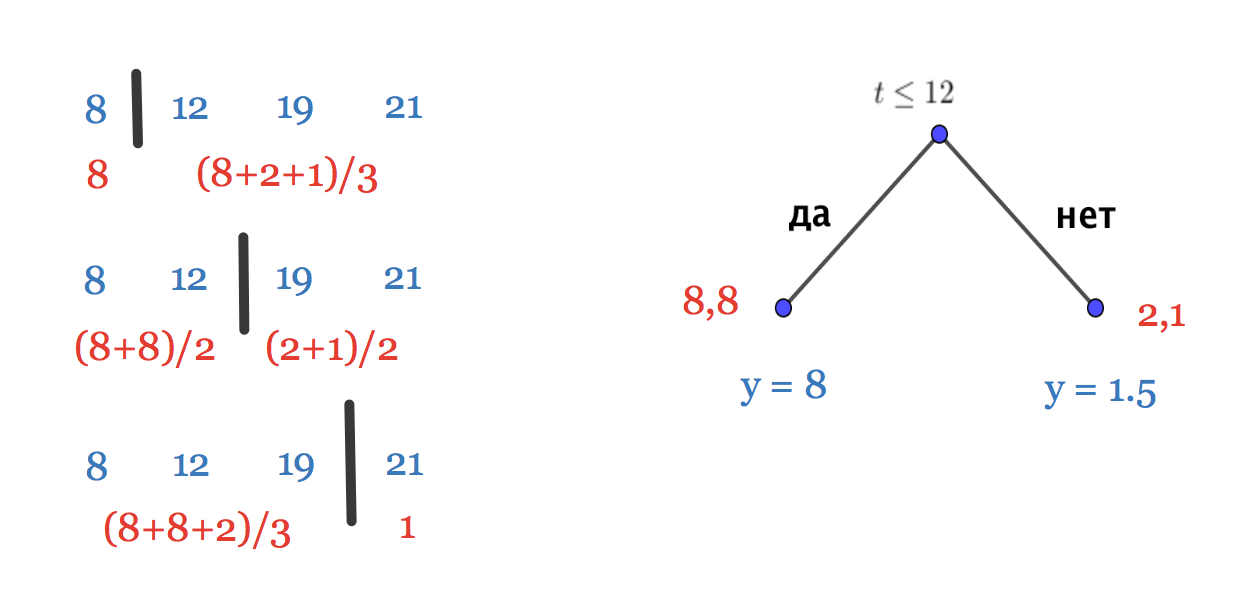
\includegraphics[scale=0.25]{reg_tree_1.png}
\end{center}
	
\begin{itemize}

    \item  	Мы можем отправить  в левую вершину все ситуации, где температура меньше либо равна 8 градусам. В таком случае, когда мы идём по дереву налево, мы будем прогнозировать, что потребители выпьют $8$ чашек кофе. Когда мы идём в правую вершину, мы будем прогнозировать, что потребители выпьют $3.6$ чашек кофе. Это среднее всех $y$, попавших в правую вершину. Давайте посчитаем ошибку, которую при этом будет допускать дерево. 

	$$
	(8 - 8)^2 + (8 - 3.6)^2 + (2 - 3.6)^2 + (1 - 3.6)^2 = 28.68.
	$$

	\item Мы можем отправить в левую вершину все ситуации, где температура меньше либо равна $12$. В таком случае слева прогноз будет $8$, а справа $1.5$. Найдём ошибку:
	
	$$
	(8 - 8)^2 + (8 - 8)^2 + (2 - 1.5)^2 + (1 - 1.5)^2 = 0.5.  $$
	
	\item В третьей ситуации получаем, что 
	
   $$ 
   (8 - 6)^2 + (8 - 6)^2 + (2 - 6)^2 + (1 - 1)^2 = 24.
   $$
\end{itemize}
	
Оптимальным для разбиения оказывается второй вариант. Он сильнее всего уменьшает ошибку.  Выбрав его, мы отправляем в левую вершину две восьмёрки и получаем в ней нулевую ошибку. В правую вершину мы отправляем двойку и единицу. 
	
В правой вершине нужно сделать ещё одну итерацию, чтобы отделить двойку от единицы. Тогда обучение дерева будет окончено. Итоговое дерево будет иметь вид: 
	
\begin{center}
	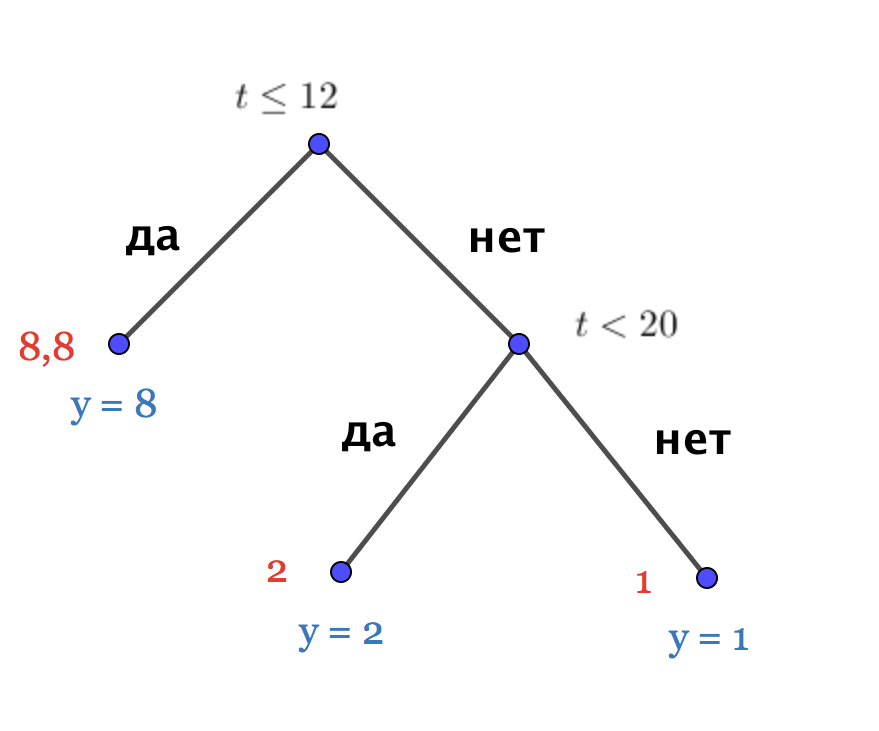
\includegraphics[scale=0.23]{reg_tree_2.png}
\end{center}

Ура! Конец. Компьютер обучает деревья ровно так, как мы сейчас сделали это руками. Правда обычно данных ему мы скармливаем намного больше. 
	
Сделаем прогноз для $13$ градусов.  Для этого пройдёмся по дереву от корня к одному из листов. На улице меньше или равно $12$ градусов?  нет. Идём направо. На улице меньше $20$ градусов? Да. Идём налево. В кофейне купят $2$ чашки. 

Можно ли для обучения использовать $MAE$? А почему собственно нет?! Попробуйте дома проделать это руками самостоятельно.

Обратите внимание, что дерево идеально запомнило обучающую выборку. Оно слишком сильно фрагментировало её. Такая ситуация, когда модель идеально вылизывает обучающие данные, называется \indef{переобучением.} Чтобы деревья не переобучались и не вылизывали выборку, обычно останавливают обучение деревьев досрочно: 
	
\begin{itemize} 
	\item  Когда в вершине оказалось не менее $10$ объектов
	\item  Когда дерево построилось до $20$ листьев. 	
	\item  Когда глубина дерева оказалась равна $5$.
\end{itemize}
	
Конечно же конкретные цифры здесь для примера. Их можно подбирать по данным. Их, кстати говоря обычно называют \indef{гиперпараметрами.} 

Ещё, чтобы деревья не переобучались, их обычно объединяют в леса. Именно этим мы с вами на следующей паре и займёмся, но уже на компьютере. 
\end{solution}


\section*{Ещё задачи} 

Тут находится несколько задачек, о которых вам нужно подумать самостоятельно. Возможно, что похожие задачи попадутся вам на самостоятельной работе.

\begin{problem}{ }
Вот несколько ситуаций, как на ваш взгляд должны пройти линии регрессии? Да, это тоже машинное обучение. Но обычно кривые рисуем не мы, а комплюхтер.

\begin{minipage}[t]{0.45\textwidth}
	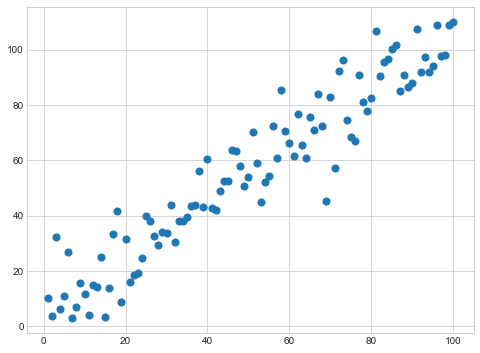
\includegraphics[scale=0.38]{regr_pic_1.png}
\end{minipage}
\hfill
\begin{minipage}[t]{0.45\textwidth}
	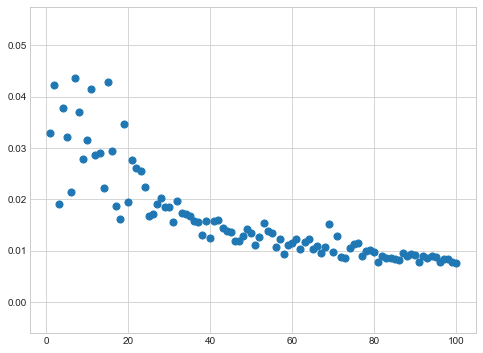
\includegraphics[scale=0.38]{regr_pic_2.png}
\end{minipage}

\begin{minipage}[t]{0.45\textwidth}
	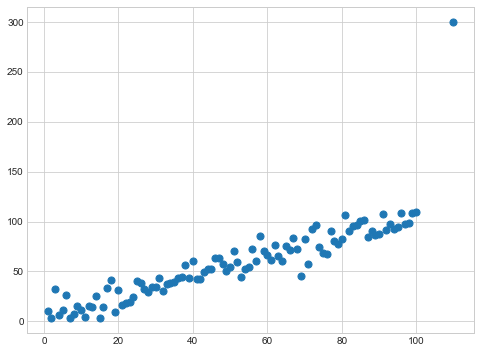
\includegraphics[scale=0.38]{regr_pic_3.png}
\end{minipage}
\hfill
\begin{minipage}[t]{0.45\textwidth}
	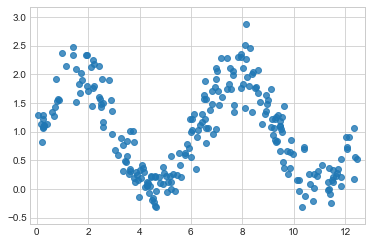
\includegraphics[scale=0.5]{regr_pic_4.png}
\end{minipage}

\begin{enumerate}	
	\item[а)] Нарисуйте на каждой из картинок линию регрессии.
	\item[б)] Как выглядят уравнения регрессии в этих ситуациях? Какие параметры в них нам нужно обучить?
	\item[в)] В чём проблема на картинке слева снизу? Проинтерпретируйте её на примере шашлыков.
	\item[г)] В четвёртой ситуации мы выбрали для обучения полином. А почему бы не взять его в каждой ситуации и не обучить через каждую точку? 
	\item[д)] Ещё одна, на этот раз трёхмерная картинка! Слабо дополнить её также, как мы делали это выше? Как будет выглядеть уравнение регрессии?
\end{enumerate}

\begin{center}
	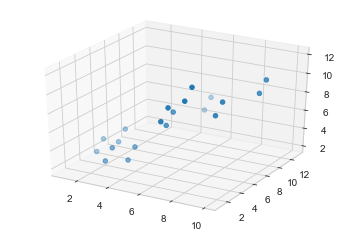
\includegraphics[scale=0.8]{regr_pic_5.png}
\end{center}
\end{problem}

\begin{solution}
	\begin{enumerate}	
		\item[а)] Берём и рисуем! 
		
		\begin{minipage}[t]{0.45\textwidth}
			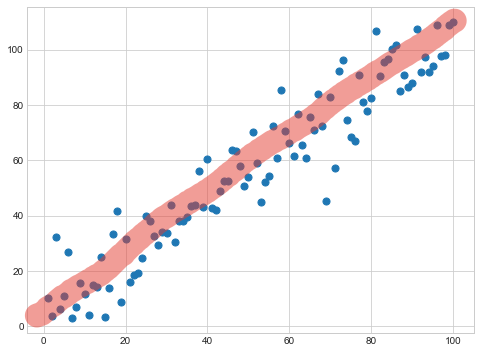
\includegraphics[scale=0.4]{regr_pic_1_ans.png}
		\end{minipage}
		\hfill
		\begin{minipage}[t]{0.45\textwidth}
			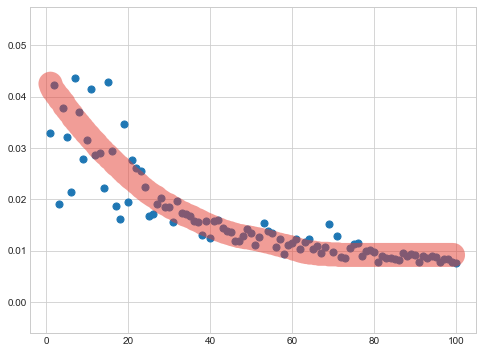
\includegraphics[scale=0.4]{regr_pic_2_ans.png}
		\end{minipage}
		
		\begin{minipage}[t]{0.45\textwidth}
			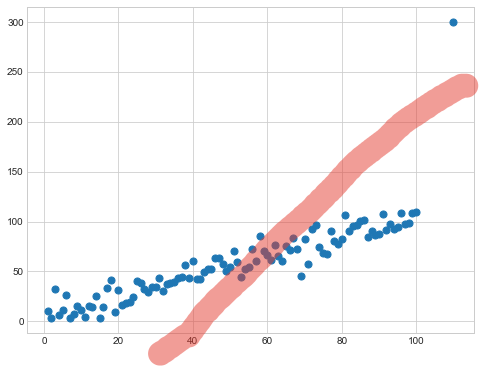
\includegraphics[scale=0.4]{regr_pic_3_ans.png}
		\end{minipage}
		\hfill
		\begin{minipage}[t]{0.45\textwidth}
			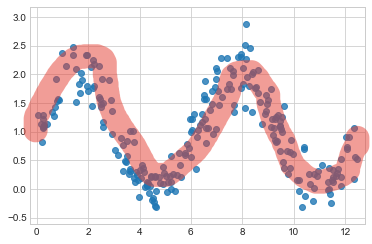
\includegraphics[scale=0.55]{regr_pic_4_ans.png}
		\end{minipage}
		
		
		\item[б)]  В первой ситуации это обычная линейная модель $y_i = \beta_0 + \beta_1 x_i$. Во второй ситуации перед  нами нелинейная модель. Внешне картинка похожа на гиперболу. Можно попробовать обучить модель $y_i = \frac{1}{\beta_0 + \beta_1 x_i}$. Однако на практике обычно поступают иначе. Если взять от $x_i$ логарифм, то модель стане линейной, и модно будет обучить $y_i = \beta_0 + \beta_1 \ln x_i$. В третьей ситуации это снова обычная линейная модель. В четвёртой ситуации это либо многочлен, либо какой-нибудь косинус. Об этих двух ситуациях мы поговорим подробнее ниже. 
		
		\item[в)]  Это толстый друг, который много ест.  Он портит обучение модели и прямая, вместо того, чтобы пройти через облако точек, подстраивается под него. Такие ситуации обычно \indef{называют выбросами.} Если последовать рецепту из первого упражнения и наложить на тостого друга дамми, то ситуация нормализируется, и красная прямая пройдёт сквозь облако также как и в первой ситуации. Это эквивалентно тому, что мы выбрасываем друга из выборки и работаем с ним отдельно.
		
		Другой путь: использовать модели, которые нечувствительны к выбросам. Например,  использовать для обучения модели $MAE$!
		
		\item[г)]  В четвёртой ситуации мы взяли полином. Возможно, у вас возник соблазн обучить и в первых трёх ситуациях модель, которая пройдёт через все возможные точки. Это неправильно. В таком случае наша модель слишком сильно вылизывает данные. Обычно в данных много шума, и модель подстраивается под него, вместо того, чтобы вычленить сигнал, \indef{то есть переобучается.} 
		
		\item[д)]  В этой ситуации мы строим модель не на одну переменную ($y$ на $x$), а на две ($y$ на $x$ и на $z$). Уравнение будет иметь вид 
		
		$$
		y_i = \beta_0 + \beta_1 \cdot x_i + \beta_2 \cdot z_i.
		$$
		
		В алгебре такое уравнение описывает двумерную плоскость в трёхмерном пространстве. Новость: в трёхмерном случае мы учим не линию, а плоскость! 
		
		\begin{center}
			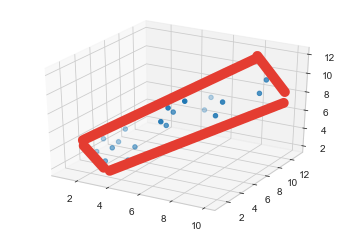
\includegraphics[scale=0.8]{regr_pic_5_ans.png}
		\end{center}
	\end{enumerate}
\end{solution}

\begin{problem}{ }
Драгомир пытается предсказать продажи видео-игр.  Для моделирования он использует две переменные: $x_1$ --- возраст игры, $x_2$ --- на кого она ориентирована. Если на мужчин, $x_2=1$, если на женщин, $x_2=0$. Целевая переменная $y$ --- количество проданных экземпляров игры. Драгомир оценил линейную регрессию: 

$$ y = 1000 - 100 \cdot  x_1 + 200 \cdot  x_2.$$

Проинтерпретируйте полученные коэффициенты.  Предположим, что мы выпускаем на рынок свежую игру для женщин. Спрогнозируйте наши продажи. 
\end{problem}

\begin{solution}
Получается, что $\beta_0 = 1000$ --- это базовые продажи, $\beta_1 = -100$ --- насколько падают продажи игры с каждым новым годом её присутствия на рынке, $\beta_2 = 200$, насколько выше продажи игр, которые ориентированны на мужчин.

Чтобы сделать прогноз, просто подставим в уравнение интересующие нас условия: 

$$ 
\hat y_{new} = 1000 - 100 \cdot 0 + 200 \cdot 0 = 1000
$$

Получится $2000$ экземпляров игры. 
\end{solution}


\begin{problem}{ }
Мстислаполк, конкурент Драгомира, тоже пытается предсказать продажи видео-игр.  Для моделирования он использует две переменные: $x$ --- возраст игры. Целевая переменная $y$ --- сумма продаж. Мстислаполк оценил линейную регрессию: 

$$ 
\ln y = 5 - 6 \cdot  \ln x.
$$

Проинтерпретируйте полученный коэффициент.  Предположим, что мы отгружаем на рынок новую партию игры, выпущенной в прошлом году. Сколько экземпляров этой игры будет продано? 
\end{problem}

\begin{solution}
Начнём с прогноза: 
$$ 
\ln \hat y_{new} = 5 - 6 \cdot \ln 1 = 5 - 0 = 5,
$$

то есть $5$ логарифмов экземпляров игры. Чтобы перейти от логарифмов игр просто к играм, надо сделать действие обратное логарифмированию. То есть взять от $5$ экспоненту: 
$$
\hat y = exp(5) \approx 148,
$$

То есть мы продадим $148$ экземпляров игры. Теперь давайте проинтерпретируем коэффициенты. Базовый логарифм продаж это $\beta_0 = 5$.  При росте возраста игры на $1\%$, продажи будут падать примерно на $6\%$. За это отвечает коэффициент $\beta_1 = 6$. 

Давайте ради интереса убедимся, что я вам не вру и продажи правда упадут на $6\%.$  Возраст игры у нас был равен $1$. Если игра станет на процент старше, получится $1.01$. Спрогнозируем $y$. Несложно посчитать, что это будет:

$$
\hat y = exp(5 - 6 \cdot \ln 1.01) \approx 140.
$$

Получается, что продажи упали на $100 \cdot \frac{148-140}{148} \approx 6\%$.
\end{solution}


\begin{problem}{}
Логарифмирование позволяет сгладить длинные хвосты распределений, кишащие выбросами. Из-за этого на практике переменные довольно часто логарифмируют. На картинке ниже изображена гистограмма продаж в супермаркетах Wallmart. По оси $x$ отложена сумма продаж, по оси $y$ число продаж на такую сумму.  

\begin{center}
	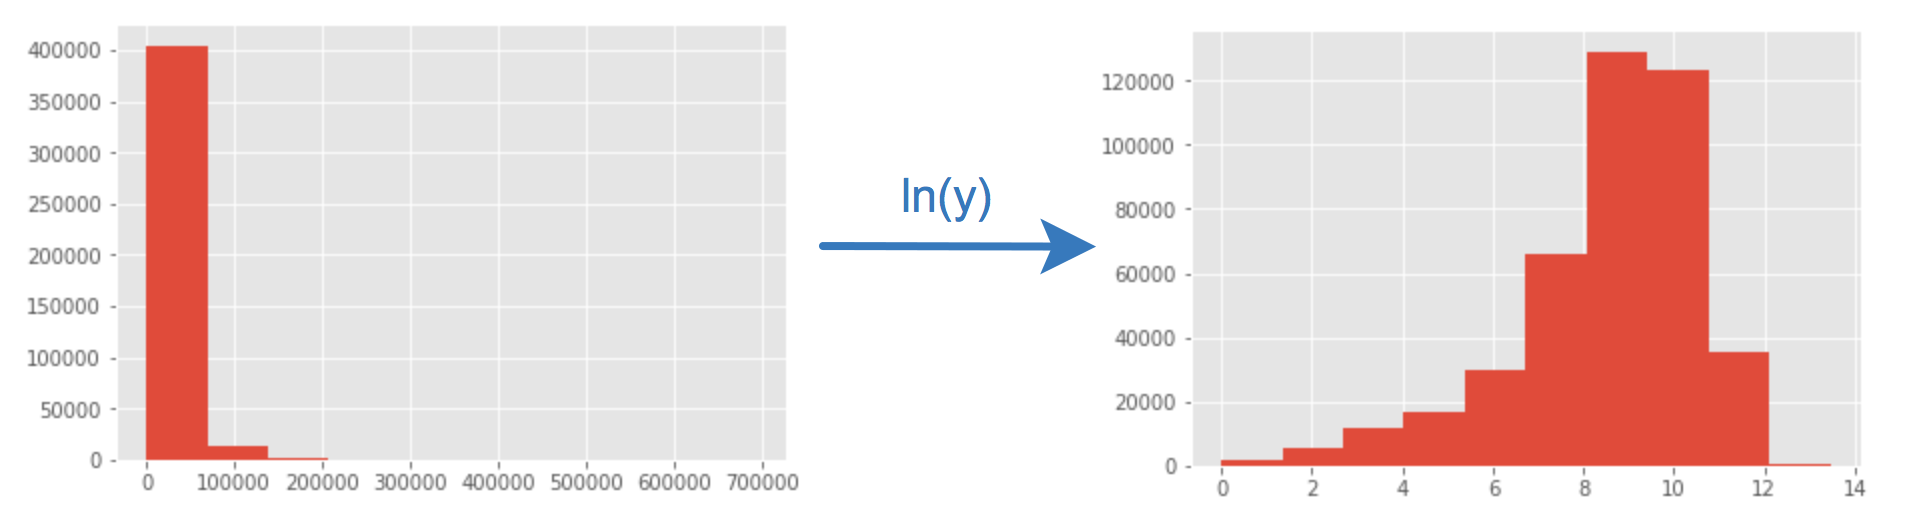
\includegraphics[scale=0.2]{y_lny.png}
\end{center}

Понятное дело, что люди делают покупки на огромные суммы, но в маленьком количестве. Отсюда у распределения появляется огромный хвост. Если прологарифмировать продажи, распределение станет няшным.

Попробуйте посмотреть как именно происходит это сглаживание. Предположим, что в магазинах продали $y_1 =100$, $y_2 = 200$, $y_3 = 300$ и $y_4 = 1000$ игр. Посчитайте разницу между соседними наблюдениями. Прологарифмируйте их. Что стало с этой разницей? 
\end{problem}

\begin{solution}
Возьмём логарифмы: 

$$
\ln y_1 = 4.6 , \ln y_2 = 5.3, \ln y_3 =5.7, \ln y_4 = 6.9.
$$

Наблюдения стали намного плотнее прилегать друг к другу. Выброс $y_4$ довольно сильно сгладился. Именно это мы видим на гистограмме выше. Посмотрим на то, что происходит c разностями между соседними наблюдениями:


\begin{align*}
    y_2 - y_1 = 100 & \qquad \ln y_2 - \ln y_1 = \ln 200 - \ln 100 = 0.69 \\
    y_3 - y_2 = 100 & \qquad \ln y_3 - \ln y_2 = \ln 300 - \ln 200 = 0.4 \\
    y_4 - y_3 = 900 & \qquad \ln y_4 - \ln y_3 = \ln 1000 - \ln 300 = 1.2 \\
\end{align*}

Между $y_1$, $y_2$ и $y_2,y_3$ до логарифмирования была одинаковая разность $(100)$. Теперь, из-за того, что логарифм сгладил хвост, $y_3$ ближе к $y_2$, чем $y_2$ к $y_1$. В принципе, если построить график с логарифмом, эти свойства видны на нём. Чем больше $x$, тем меньший прирост по $y$ происхоит.

\begin{center}
\begin{tikzpicture}[line cap=round,line join=round,x=1.0cm,y=1.0cm]
    \draw [->,line width=1.5pt] (-0.5,0) -- (8,0);
    \draw [->,line width=1.5pt] (0,-2) -- (0,3.5);
    \draw [blue, thick, domain=0.3:7] plot (\x, {log2(\x)});
    \draw (8,-0.2) node[anchor=north west] {$x$};
    \draw (-1,4.3) node[anchor=north west] {$f(x) = \ln x$};
\end{tikzpicture}
\end{center}
	
Такие вот у логарифма классные свойства. Конечно же, \indef{логарифмирование не всегда спасает от длинных хвостов,} но иногда оно бывает довольно полезным. 
\end{solution}


\begin{problem}{ }
В один прекрасный день Маша проснулась в своей кровати и поняла, что она и есть та самая маша, которой принадлежит лёрнинг. Она решила посвятить машин лёрнингу всю свою жизнь и стала коллекционировать модели.

Вчера она пообщалась с Мишей. Он тоже коллекционер. Он спросил у неё, какое у её моделей качество. Маша не смогла ответить. Ей было очень стыдно\footnote{Прям как вам после самостоятельной на следущей паре}. Она решила проверить качество. У неё есть три наблюдения $y_i$. Она для каждого построила прогнозы. Найдите для её прогнозов $MAE$, $MSE$, $RMSE$ и $MAPE$. 

\begin{center}
	\begin{tabular}{c|c|c|c}
		настоящие $y_i$ &  1 & 2 & 3 \\
		\hline
		прогнозы нейросети & 2 & 3 & 1  \\
		прогнозы регрессии &  2 & 3 & 4 \\
		прогнозы случайного леса & 1 & 1 & 1 \\
	\end{tabular}
\end{center}
\end{problem}


\begin{problem}{ }
Объясните мемас: 

\begin{center}
	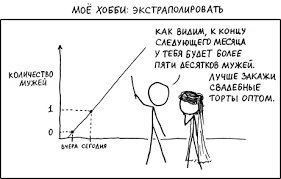
\includegraphics[scale=0.8]{memes.png}
\end{center}
\end{problem}


\begin{problem}{}
Выращиваем регрессионное дерево в домашних условиях! Вот вам выборка для этого: 

\begin{center}
	\begin{tabular}{c|c}
		$x_i$ & $y_i$ \\
		\hline
		0 & 5 \\
		1 &  6\\
		2 & 4 \\
		3 & 100 \\
	\end{tabular}
\end{center}

Критерий деления вершины --- минимизация квадратичной функции потерь $(MSE)$. Критерий остановки --- три листа.  Зачем нужен критерий остановки? Как дерево ведёт себя с выбросами? 
\end{problem}

\begin{solution}
У нас есть три способа раздробить по $x$ дерево. 

\begin{center}
	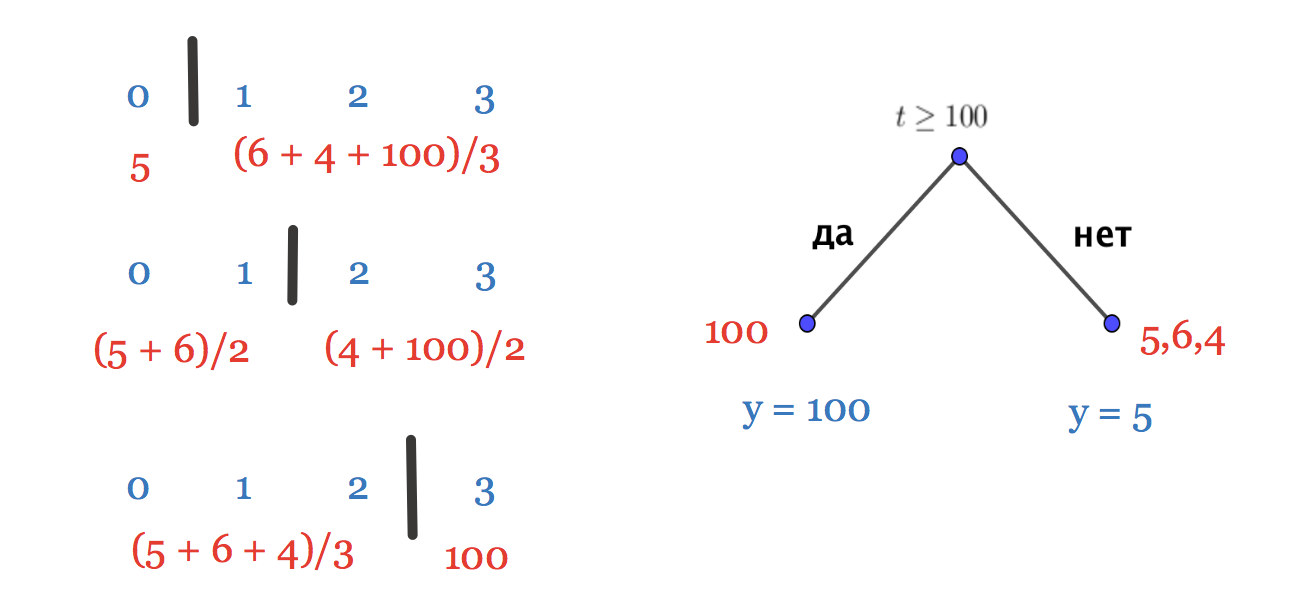
\includegraphics[scale=0.25]{reg_tree_3.png}
\end{center}

Посчитаем для каждого способа квадратичную ошибку: 

\begin{itemize}
	\item  $ (5 - 5)^2 + (6 - 36.6)^2 + (4 - 36.6)^2 + (100 - 36.6)^2 = 6018.68$
	\item  $ (5 - 5.5)^2 + (6 - 5.5)^2 + (4 - 52)^2 + (100 - 52)^2 = 4608.5$
	\item  $ (5 - 5)^2 + (6 - 5)^2 + (4 - 5)^2 + (100 - 100)^2 = 2$
\end{itemize}

Выгоднее всего оказывается обособить первым же отсечением выброс. Это нормальная ситуация. На практике так происходит регулярно. \indef{Деревья изолируют выбросы в отдельные вершины, и они никак не портят работу с основной выборкой. Такое свойство называется нечувствительностью к выбросам или робастностью к выбросам.} 

Сделаем второй шаг разбиения. 

\begin{center}
	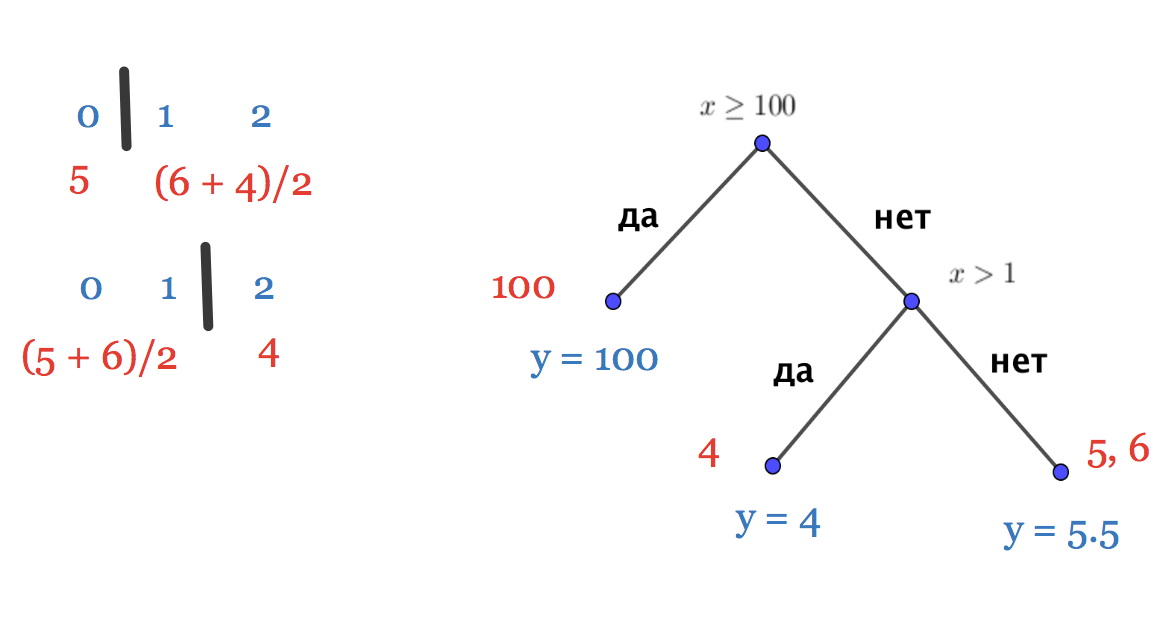
\includegraphics[scale=0.25]{reg_tree_4.png}
\end{center}

Посчитаем для каждого способа квадратичную ошибку: 

\begin{itemize}
	\item  $ (5 - 5)^2 + (6 - 5)^2 + (4 - 5)^2 = 2$
	\item  $ (5 - 5.5)^2 + (6 - 5.5)^2 + (4 - 4)^2  = 0.5$
\end{itemize}
	
Понятно, что дробить нужно, обосабливая четвёрку. После этого нужно остановиться. По условию задачи критерий остановки --- три листа у дерева. Ошибка бы продолжила убывать для тренировочной выборки. На тестовой она бы возрастала. Обычно подобные критерии ранней остановки помогают избежать переобучения.
	
Кстати говоря, именно благодаря тому, что деревья на первом же шаге изолируют выбросы, случайный лес можно из прогнозной модели модернизировать в модель, которая неплохо справляется с поиском аномалий. Подумайте на досуге о том, как именно можно сделать это. 
\end{solution}


\begin{problem}{ }
В какой	из следующих ситуаций какую метрику качества вы бы использовали?  Почему? Постарайтесь чётко обосновать свой выбор с точки зрения физического смысла задачки. Для удобства будем в каждом пункте обозначать наблюдаемый спрос/цену/вес и тп как  $y_i$, а наши прогнозы как  $\hat y_i$.

\todo[inline]{Примеры странные какие-то тут. Мб выкинуть это упражнение?}

\begin{itemize} 
\item Марк и Семён решили накачаться. У них есть модель, которая прогнозирует их набор массы в зависимости от рациона. По вердиктам этой модели парни заказывают себе еду на неделю. В конце недели они взвешиваются и смотрят насколько сильно модель ошиблась.
	
\item Коста собирается устроить вечеринку. Для неё ему понадобится шашлык  (внезапно). Есть моделька, которая позволяет прикинуть сколько шашлыка ему понадобится. Он построил прогнозы для прошлой вечеринки и задумался о том какую метрику нужно выбрать для оценки качества её работы. На прошлой тусе ели только шашлык. На этой тусе, кроме шашлыка будет ещё и пицца.  Предположим, что у Косты есть один толстый друг. Возможно, он будет есть шашлык, но вот вообще не факт. 

\item  Кот Матроскин продаёт молоко. Каждую неделю он прогнозирует спрос на молоко и поставляет его в торговые точки в соответствии с прогнозами. Каждая бутылка продаётся за $40$ рублей. Если он завозит слишком много, молоко портится и Матроскин теряет деньги, потраченные на производство молока и различные логистические издержки (перевозка и т.п.). Потери составляют $60$ рублей с каждой просроченной бутылки. 
	
\item Мистер Белфорд торгует на бирже. Каждую неделю он отсчитывается перед инвесторами, рассказывая сколько дополнительных процентов от стартовых инвестиций принёс его алгоритм торговли. Внутрь алгоритма вшита прогнозная модель. Как лучше всего мистер Белфорд мог бы оценить её качество? 
\end{itemize} 
\end{problem}

\end{document}